%!TEX root=ast2016.tex

\begin{figure*}[t]
  \centering

  \begin{tabular}{c c}

    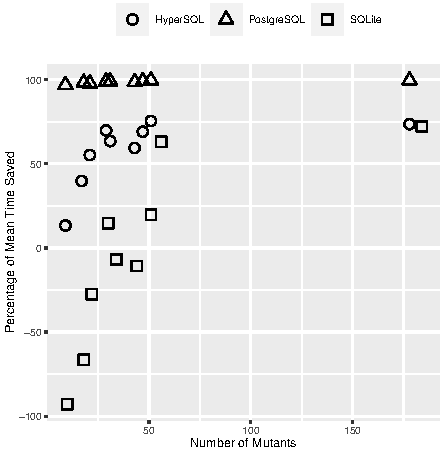
\includegraphics[scale=1.0]{graphics/graphic_scatterplot_nummutants_percentage.pdf} &
    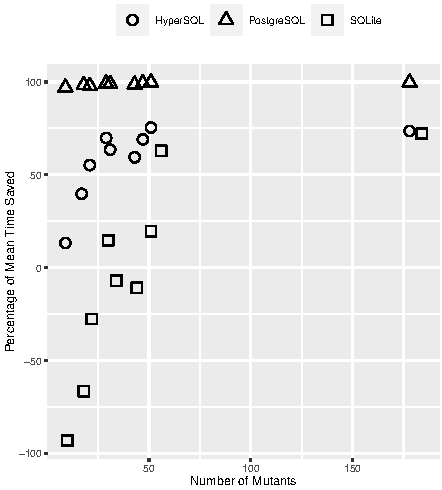
\includegraphics[scale=1.0]{graphics/graphic_scatterplot_numtests_percentage.pdf}

  \end{tabular}

  % Analysis of the results in this output (number of mutants):

  % - Make sure that the paper gives the equation that was used to calculate the percentage savings.
  % - Note that I did not screen out the results where there is no savings because virtual is more expensive (Chris does
  %   this in his code, if I am understanding that code correctly).
  % - For any number of mutants, there is always a high percentage savings for the Postgres DBMS; for this DBMS the
  %   percentage increases slightly as the number of mutants increases.
  % - The HyperSQL DBMS always shows percentage of time saved that is positive.
  % - But, for HyperSQL, the percentage savings is gradual and it tapers off around 75 percent for the greatest number of
  %   mutants.
  % - For SQLite, the percentage savings is negative (meaning that it takes longer to use the virtual technique, as
  %   mentioned in the previous analysis). But, the absolute increase in time is modest for these cases.
  % - There are four schemas (check which ones) for which there is a positive percentage savings for SQLite.
  % - Note that when the schema is large, the percentage savings for SQLite is similar to that for HyperSQL. Again, this
  %   demonstrates that the virtual technique is always useful when doing mutation testing of large schemas.

  % Analysis of the results in this output:

  % - The trends in this graph are similar to what was given for the previous graph.
  % - This graph should only be included as space is available, place near the other graph.

  \caption{Scatter plot of the percentage of mean time saved for the number of mutants (left) and tests (right).}
  \label{fig:graphic_scatterplot_mutantstests_percentagetimesaved}

  {\small \justifying{ \noindent In these scatter plots, a given point corresponds to the percentage of mean time saved
      for a given number of mutants (left plot) or tests (right plot), across all three of the DBMSs. The percentage of
      mean time save is determined by first calculating the mean execution time from the thirty trials of both the
      standard and the virtual techniques. If $T_s$ denotes the time taken by the standard method and $T_v$ is the time
  needed to run the virtual one, then the percentage of mean time saved shown on the vertical axis is given by $({T_s
  - T_v})/{T_s}$. } \par}

\end{figure*}
